\chapter{Experiments}
Recall an FMCW radar system has several configurable parameters, including the
chirp rate $\alpha$, the chirp period $T_c$, and the number of chirps $K$ in a chirp
frame. To verify the FMCW radar mathematics and investigate
the effects of these parameters, we ran several simulations in Python.

For these simulations we modeled the radar system after Texas Instruments's
IWR 1443 FMCW chip, which has a carrier frequency $f_c$ of 77 GHz and a sampling
frequency of 3 Msps \cite{iwr1443datasheet}. We will use a 256-point FFT for the
range-FFT and a 32-point FFT for the Doppler-FFT. For these simulations, we are just investigating the
range-FFT and Doppler-FFT behavior, so we simplify the model to have a single
transmit-receive antenna pair. Additionally, we will assume we have ideal point
targets with no attenuation to better isolate the effects of the system
parameters within the simulations. We will simulate three targets with different
ranges and velocities, as shown in Table \ref{tab:targets}. For this
model, we also include additive white Gaussian noise on the received signal.

\begin{table}[h]
	\centering
	\begin{tabular}{l|c|c}
		Target & Range & Velocity \\
		\hline
		Target 1 & $5.0 m$ & $0 m/s$ \\
		Target 2 & $10.0 m$ & $5.0 m/s$ \\
		Target 3 & $20.0 m$ & $-7.5 m/s$ 
	\end{tabular}
	\caption{Simulated target initial positions and velocities}
	\label{tab:targets}
\end{table}

We will consider a baseline case with a chirp period of 60 $\mu$s, a
bandwidth of 500 MHz, 30 chirps per chirp frame, a 256-point range-FFT,  and a
32-point Doppler-FFT. As the bandwidth, chirp period, and chirp rate are
intrinsically linked, we only need to define two parameters to determine all
three. These parameters give a range resolution of 21.1 cm, a maximum distance
of 53.79 m, a velocity resolution of 1.01 m/s, and a velocity range of $\pm$15.2
m/s. Figure \ref{fig:baseline} shows the range-FFT for a single chirp and the
range-Doppler plot for this parameter selection. We can clearly see three peaks
in both plots, corresponding to the three targets. The recovered distances were
5.06 m, 10.13 m, and 19.83 m. Likewise, the recovered velocities were 0.0 m/s,
5.07 m/s, and -7.10 m/s.

\begin{figure}[h]
	\centering 
	\begin{subfigure}[c]{0.5\textwidth}
		\centering
		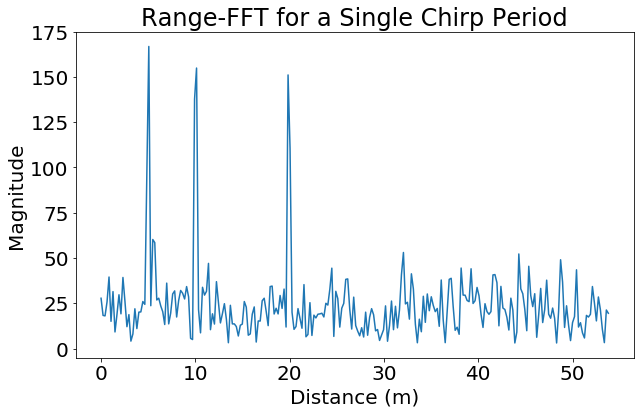
\includegraphics[width=2.5in]{imgs/baseline_range}
		\caption{Range-FFT for a single chirp with the baseline
		parameters}
	\end{subfigure}%
	~
	\begin{subfigure}[c]{0.5\textwidth}
		\centering
		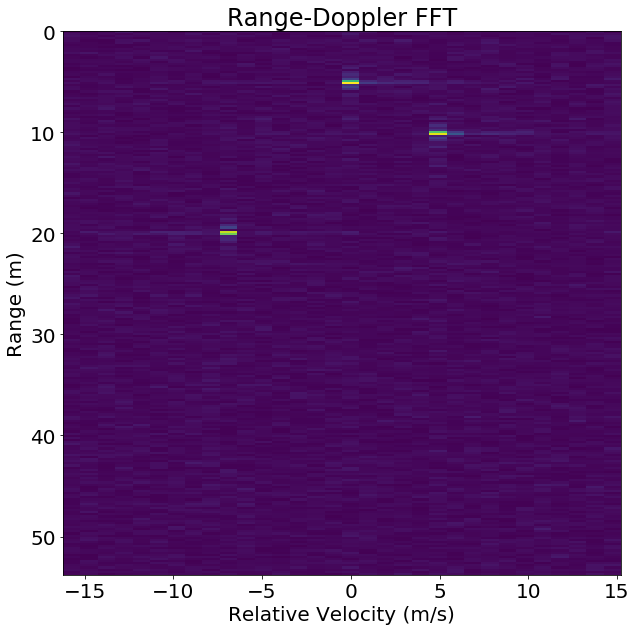
\includegraphics[width=2.5in]{imgs/baseline_doppler}
		\caption{Dopper-FFT for the baseline parameters}
	\end{subfigure}
	\caption{Baseline simulation results}
	\label{fig:baseline}
\end{figure}

Now consider the case where the bandwidth is doubled to $1 GHz$ while
maintaining the same chirp period. This clearly doubles the chirp rate, giving
us a range resolution of 10.5 cm, but a maximum distance of only 26.9 m, keeping
the other parameters the same from the baseline simulation. We can see from the
results shown in Figure \ref{fig:bandwidth} that we still have three clear
peaks corresponding to the targets, with recovered distances 4.96 m, 10.02 m,
and 19.93 m and corresponding recovered velocities of 0.0 m/s, 5.07 m/s, and
-7.10 m/s. Though both plots show the improved range resolution, the
range-Doppler plot more clearly shows the range resolution change as the pixel
widths corresponding the range bins are more clearly demarcated.  

\begin{figure}[h]
	\centering 
	\begin{subfigure}[c]{0.5\textwidth}
		\centering
		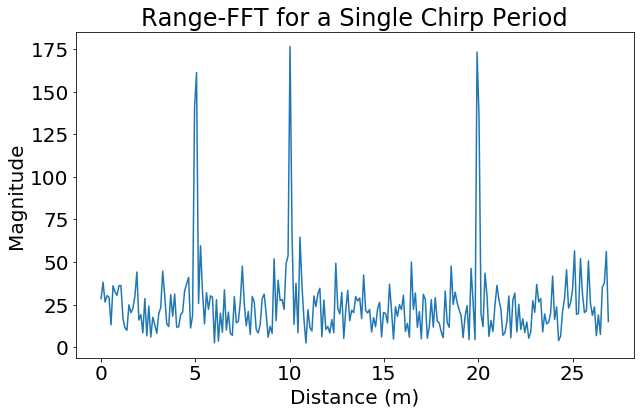
\includegraphics[width=2.5in]{imgs/bandwidth_range}
		\caption{Range-FFT for a single chirp with 1 GHz bandwidth}
	\end{subfigure}%
	~
	\begin{subfigure}[c]{0.5\textwidth}
		\centering
		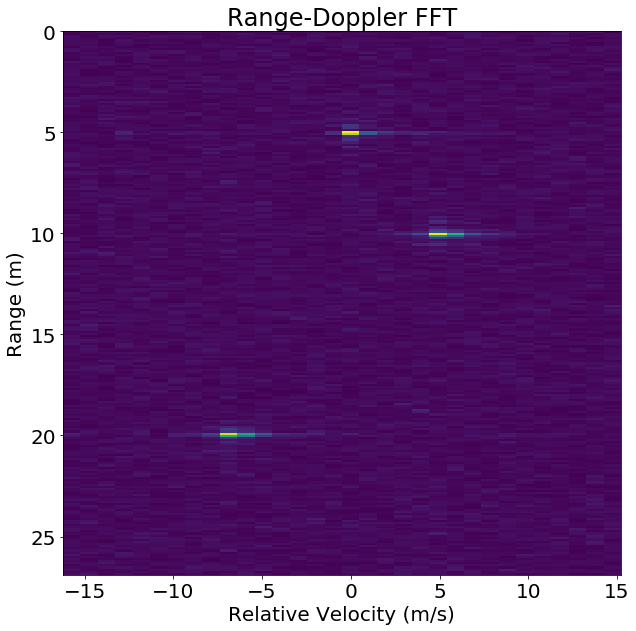
\includegraphics[width=2.5in]{imgs/bandwidth_doppler}
		\caption{Dopper-FFT for the 1 GHz bandwidth version of the
		baseline system}
	\end{subfigure}
	\caption{Increased bandwidth simulation results}
	\label{fig:bandwidth}
\end{figure}

To see the effect of the chirp period, let us examine the baseline system with
the chirp period doubled to 120 $\mu$s. With a bandwidth of 500 MHz, this halves
the chirp rate of the baseline system. By halving the chirp rate, our range
resolution decreases to 42.2 cm and the maximum range increases to 107.6 m. We
also see the velocity resolution improve to 0.51 m/s but the velocity range is
halved to $\pm$7.61 m/s. Figure $\ref{fig:period}$ shows the simulations
results, with recovered distances 5.06 m, 10.13 m, and 19.83 m. We see that the
Doppler-FFT recovers two clean peaks for the first two targets, with recovered
velocities 0.0 m/s and 5.07 m/s respectively. However, due to the FFT smearing, the second target's
velocity of -7.5 m/s is split between two peaks recovered at -7.61 m/s and -7.1
m/s.

\begin{figure}[h]
	\centering 
	\begin{subfigure}[c]{0.5\textwidth}
		\centering
		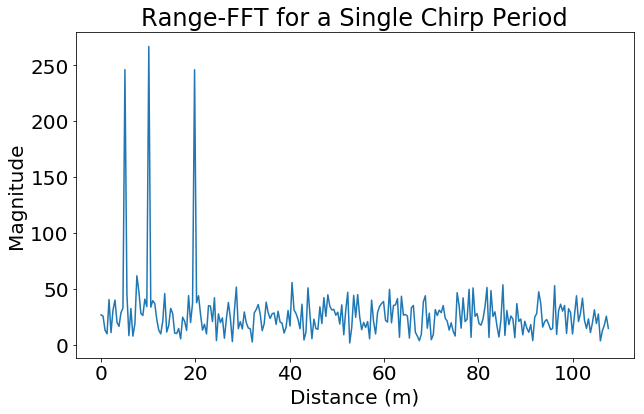
\includegraphics[width=2.5in]{imgs/long_period_range}
		\caption{Range-FFT for a single chirp with period 120 $\mu$s}
	\end{subfigure}%
	~
	\begin{subfigure}[c]{0.5\textwidth}
		\centering
		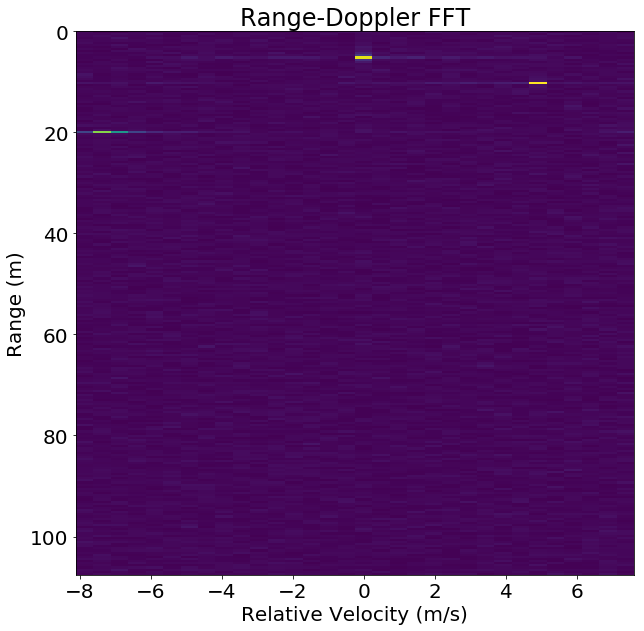
\includegraphics[width=2.5in]{imgs/long_period_doppler}
		\caption{Dopper-FFT for 120 $\mu$s chirp period system
		system}
	\end{subfigure}
	\caption{Increased chirp period simulation results}
	\label{fig:period}
\end{figure}

Now, if we replicate the baseline system, except with a chirp frame of only 15
chirps, we expect to only see a difference in the Doppler results. In fact, we
can clearly see the sinc function in the Doppler-FFT in Figure \ref{fig:chirps}, as we
are padding the input signal of length 15 (number of chirps) to be length 32 for
the FFT. This increase in zero-padding from the baseline case more clearly shows
the Doppler-FFT sampling on the non-zero points of the rectangle window
spectrum, causing this spectrum leakage. Choosing a different windowing
function, such as the Hamming window could help alleviate this spectral leakage,
though more investigation into the proper window choice is still required.

\begin{figure}[h]
	\centering 
	\begin{subfigure}[c]{0.5\textwidth}
		\centering
		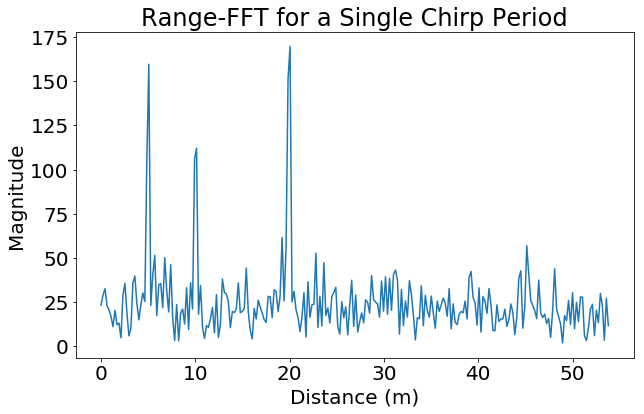
\includegraphics[width=2.5in]{imgs/chirps_range}
		\caption{Range-FFT for a single chirp}
	\end{subfigure}%
	~
	\begin{subfigure}[c]{0.5\textwidth}
		\centering
		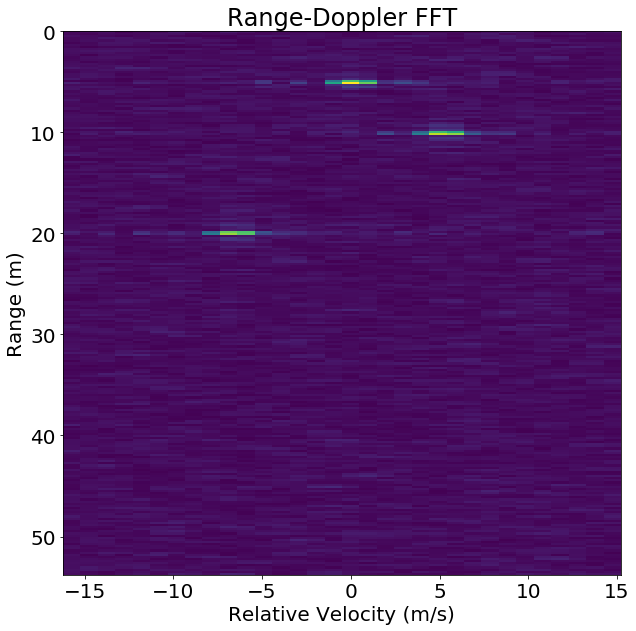
\includegraphics[width=2.5in]{imgs/chirps_doppler}
		\caption{Dopper-FFT for 15 chirps/frame system}
	\end{subfigure}
	\caption{Decreased number of chirps per frame results}
	\label{fig:chirps}
\end{figure}

Table \ref{tab:simulation} provides a summary of the different scenarios
simulated here.

\begin{table}[h] 
	\centering
	\begin{tabular}{l|c|c|c|c}
		Simulation & Bandwidth & Chirp Period & Chirp Rate & Number of
		Chirps \\
		\hline
		Baseline&500 MHz&60 $\mu$s&8.33 MHz/$\mu$s&30\\
		Bandwidth&\bf{1 GHz}&60 $\mu$s&\bf{16.67 MHz/$\mu$s}&30\\
		Chirp Period&500 MHz&\bf{120 $\mu$s}&\bf{4.167 MHz/$\mu$s}&30\\
		Chirp Number&500 MHz&60 $\mu$s&8.33 MHz/$\mu$s&\bf{15}\\
	\end{tabular}
	\caption{List of simulation parameters}
	\label{tab:simulations}
\end{table}	
